% --------------------------------------------------- %
%	Modelo para elaboração do Projeto de Graduação	  %		
%	do curso de Engenharia Elétrica - UFES			  %
%													  %
%	Adaptado do modelo de trabalho acadêmico 'abntex2'%
%	em 27/10/2016									  %
% --------------------------------------------------- %

\documentclass[
	% -- opções da classe memoir --
	12pt,				% tamanho da fonte
	openright,			% capítulos começam em pág ímpar (insere página vazia caso preciso)
	oneside,			% para impressão em recto e verso. Oposto a oneside
	a4paper,			% tamanho do papel. 
	% -- opções da classe abntex2 --
	chapter=TITLE,		% títulos de capítulos convertidos em letras maiúsculas
	section=TITLE,		% títulos de seções convertidos em letras maiúsculas
	%subsection=TITLE,	% títulos de subseções convertidos em letras maiúsculas
	%subsubsection=TITLE,% títulos de subsubseções convertidos em letras maiúsculas
	% -- opções do pacote babel --
	english,			% idioma adicional para hifenização
	french,				% idioma adicional para hifenização
	spanish,			% idioma adicional para hifenização
	brazil				% o último idioma é o principal do documento
	]{abntex2}

% --------------------------------------------------- %
% 					Pacotes básicos 				  %
% --------------------------------------------------- %
\usepackage{lmodern}			% Usa a fonte Latin Modern			
\usepackage[T1]{fontenc}		% Selecao de codigos de fonte.













































































\usepackage[utf8]{inputenc}		% Codificacao do documento (conversão automática dos acentos)
\usepackage{lastpage}			% Usado pela Ficha catalográfica
%\usepackage{indentfirst}		% Indenta o primeiro parágrafo de cada seção.
\usepackage{color}				% Controle das cores
\usepackage{graphicx}			% Inclusão de gráficos
\usepackage{microtype} 			% para melhorias de justificação
\usepackage{amsmath}
\usepackage[table,xcdraw]{xcolor} 
\usepackage{multirow}			% Para usar a tabela gerada no www.tablesgenerator.com
\usepackage{lscape} %serve para inserir página no modo paisagem
\usepackage{pdflscape} %serve para inserir página no modo paisagem
\usepackage{subfig}
\usepackage{subfloat}
% >> Pacotes de citações
\usepackage[brazilian,hyperpageref]{backref}	 % Paginas com as citações na bibl
\usepackage[alf]{abntex2cite}	% Citações padrão ABNT
%\usepackage{pgfgantt}
\usepackage{url}
% >> Configuração dos pacotes de citações
	% ---
	% Configurações do pacote backref
	% Usado sem a opção hyperpageref de backref
	\renewcommand{\backrefpagesname}{Citado na(s) página(s):~}
	% Texto padrão antes do número das páginas
	\renewcommand{\backref}{}
	% Define os textos da citação
	\renewcommand*{\backrefalt}[4]{
		\ifcase #1 %
			Nenhuma citação no texto.%
		\or
			Citado na página #2.%
		\else
			Citado #1 vezes nas páginas #2.%
		\fi}%
 
% >>> Insere a pasta onde estão contidas as figuras <<<
\graphicspath{{imagens/}}

% --------------------------------------------------- %
%		Redefinição e criação de comandos 			  %
% --------------------------------------------------- %
	
% >>> Mudar tamanho da fonte dos capítulos <<<
\renewcommand*{\chapnumfont}{\normalfont\large\bfseries\sffamily}
\renewcommand*{\chaptitlefont}{\normalfont\large\bfseries\sffamily}

\usepackage{titlesec}
\titleformat{\section}
  {\normalfont\normalsize\bfseries}{\thesection}{1em}{}
\titleformat{\subsection}
  {\normalfont\normalsize\bfseries}{\thesubsection}{1em}{}

% >>> Mudar tamanho da fonte das legendas <<<
\usepackage[font=footnotesize]{caption}

% >>> Definição do tipo CRONOGRAMA <<<
% e.g.:
% \begin{cronograma}[!h]
% 		Insira o cronograma aqui! (tabela)
% \eng{cronograma}
\newcommand{\cronogramaname}{Cronograma}
\newcommand{\listofcronogramasname}{Lista de Cronogramas}

\newfloat[chapter]{cronograma}{loc}{\cronogramaname}
\newlistof{listofcronogramas}{loc}{\listofcronogramasname}
\newlistentry{cronograma}{loc}{0}

\counterwithout{cronograma}{chapter}
\renewcommand{\cftcronogramaname}{\cronogramaname\space} 
\renewcommand*{\cftcronogramaaftersnum}{\hfill--\hfill}

% >>> Definição do tipo QUADRO <<<
% e.g.:
% \begin{quadro}[!h]
%  Insira aqui o quadro (tabela)
% \end{quadro} 
\newcommand{\quadroname}{Quadro}
\newcommand{\listofquadrosname}{Lista de Quadros}

\newfloat[chapter]{quadro}{loq}{\quadroname}
\newlistof{listofquadros}{loq}{\listofquadrosname}
\newlistentry{quadro}{loq}{0}

\counterwithout{quadro}{chapter}
\renewcommand{\cftquadroname}{\quadroname\space} 
\renewcommand*{\cftquadroaftersnum}{\hfill--\hfill}

% >>> Comando para inserir a fonte em figuras <<<
% e.g.:
% \begin{figure}[!h]
%	\centering
%	\caption{Legenda da Figura.}
%	\includegraphics[width=0.7\textwidth]{figura.jpg}
%	\source[\citeonline{Referencia}.]
%	\label{fig:label_da_figura}
%  \end{figure}
%
% Obs.: Se utilizar apenas "\source", será inserido
%       "Produção do próprio autor."


\newcommand{\source}[1][Produção do próprio autor.]{\begin{flushleft}\footnotesize Fonte: #1\end{flushleft}}

% --------------------------------------------------- %
%		Informações para personalização da capa		  %
% --------------------------------------------------- %
\newcommand{\universidade}{Universidade Federal do Espírito Santo}
\newcommand{\centro}{Centro Tecnológico}
\newcommand{\departamento}{Departamento de Engenharia Elétrica}
\newcommand{\disciplina}{Proposta de Projeto de Graduação}
\newcommand{\imprimirINSTITUICAO}{
	\MakeUppercase{\universidade} \\
	\MakeUppercase{\centro} \\
	\MakeUppercase{\departamento} \\
	\MakeUppercase{\disciplina} \\
}
% --------------------------------------------------- %
%		Informações para capa e folha de rosto		  %
% --------------------------------------------------- %
\titulo{Automação de Emprétimos de Equipamentos do Laboratório}
\autor{Lucas Soares Pessini}
\local{Vitória-ES}
\data{Junho/2019}
\orientador{Prof. Dr. André Ferreira}
\coorientador{Profa. Dra. Carla César Martins Cunha}
\instituicao{%
	\universidade
  	\par
	\centro
  	\par
	\departamento
	\par
	\disciplina
	\par}
\tipotrabalho{Proposta de Projeto de Graduação}
% O preambulo deve conter o tipo do trabalho, o objetivo, 
% o nome da instituição e a área de concentração 
\preambulo{Parte manuscrita da Proposta de Projeto de Graduação do aluno \imprimirautor, apresentada ao Departamento de Engenharia Elétrica do Centro Tecnológico da Universidade Federal do Espírito Santo, como requisito parcial para aprovação na disciplina “ELE08552 – Projeto de Graduação I”.}

% --------------------------------------------------- %
%		Configurações do aspecto final do PDF		  %
% --------------------------------------------------- %
% >> Alterando o aspecto da cor azul
\definecolor{blue}{RGB}{41,5,195}
% Informações do PDF
\makeatletter
\hypersetup{
     	%pagebackref=true,
		pdftitle={\@title}, 
		pdfauthor={\@author},
    	pdfsubject={\imprimirpreambulo},
	    pdfcreator={LaTeX with abnTeX2},
		pdfkeywords={abnt}{latex}{abntex}{abntex2}{trabalho acadêmico}, 
		colorlinks=true,       		% false: boxed links; true: colored links
    	linkcolor=black,          	% color of internal links
    	citecolor=black,        		% color of links to bibliography
    	filecolor=magenta,      		% color of file links
		urlcolor=black,
		bookmarksdepth=4
}
\makeatother

% --------------------------------------------------- %
%		Espaçamentos entre linhas e parágrafos 		  %
% --------------------------------------------------- %
% >> O tamanho do parágrafo é dado por:
\setlength{\parindent}{0cm}
% >> Controle do espaçamento entre um parágrafo e outro:
\setlength{\parskip}{18pt}

% --------------------------------------------------- %
%				Compila o Índice 					  %
% --------------------------------------------------- %
\makeindex

% --------------------------------------------------- %
%				Início do Documento					  %
% --------------------------------------------------- %

\begin{document}

% >>> Seleciona o idioma do documento (conforme pacotes do babel)
% \selectlanguage{english}
\selectlanguage{brazil}

% >>> Retira espaço extra obsoleto entre as frases.
\frenchspacing 

% --------------------------------------------------- %
%				Elementos Pré-Textuais				  %
% --------------------------------------------------- %
% \pretextual

% --------------------------------------------------- %
%						Capa						  %
% --------------------------------------------------- %
% >>> Capa Personalizada
\renewcommand{\imprimircapa}{%
	\begin{capa}%
		\center
		{\ABNTEXchapterfont\bfseries\large\imprimirINSTITUICAO}
			\vspace*{1.5cm}
		\includegraphics*[width=0.25\textwidth]{brasao_ufes.jpg}
			\vspace*{1.5cm} \\
		{\ABNTEXchapterfont\Large\imprimirautor}
				\vspace*{2.5cm} \\
		{\ABNTEXchapterfont\bfseries\Large\imprimirtitulo}
			\vfill
			\vspace*{0.5cm}
		{\large\imprimirlocal}
		\par
		{\large\imprimirdata}
			\vspace*{1cm}
	\end{capa}
}

\imprimircapa

% --------------------------------------------------- %
%					Folha de Rosto 					  %
% --------------------------------------------------- %
% >> O * indica que haverá a ficha bibliográfica

\renewcommand{\imprimirfolhaderosto}{

\begin{folhaderosto}
	\begin{center}
    	{\ABNTEXchapterfont\large\imprimirautor}
		    \vspace*{\fill}\vspace*{\fill}
    	\begin{center}
	    	\ABNTEXchapterfont\bfseries\Large\imprimirtitulo
	    \end{center}
    		\vspace*{\fill}
    		\hspace{.45\textwidth}
	    \begin{minipage}{.5\textwidth}
        	\imprimirpreambulo
	        \assinatura{\textbf{\imprimircoorientador}\\ Professora da disciplina}
	        \assinatura{\textbf{\imprimirorientador} \\ Orientador} 
			%\assinatura{\textbf{Profa. Dra. Fulana}  \\ Coorientador}
			\assinatura{\textbf{Lucas Soares Pessini}  \\ Aluno}
	    \end{minipage}
    		\vspace*{\fill}
	    \end{center}  
        \begin{center}
        	% >> Se necessáiro, ajustar os \vspace
        	%\vspace*{0.5cm}
        {\large\imprimirlocal}
        \par
        {\large\imprimirdata}
       		%\vspace*{1cm}
      \end{center}
\end{folhaderosto}
}

\imprimirfolhaderosto

% --------------------------------------------------- %
%					Ficha Catalográfica 			  %
% --------------------------------------------------- %

% Isto é um exemplo de Ficha Catalográfica, ou ``Dados internacionais de
% catalogação-na-publicação''. Você pode utilizar este modelo como referência. 
% Porém, provavelmente a biblioteca da sua universidade lhe fornecerá um PDF
% com a ficha catalográfica definitiva após a defesa do trabalho. Quando estiver
% com o documento, salve-o como PDF no diretório do seu projeto e substitua todo
% o conteúdo de implementação deste arquivo pelo comando abaixo:
%
% \begin{fichacatalografica}
%     \includepdf{fig_ficha_catalografica.pdf}
% \end{fichacatalografica}

%\begin{fichacatalografica}
%	\sffamily
%	\vspace*{\fill}					% Posição vertical
%	\begin{center}					% Minipage Centralizado
%	\fbox{\begin{minipage}[c][8cm]{13.5cm}		% Largura
%	\small
%	\imprimirautor
%	%Sobrenome, Nome do autor
%	
%	\hspace{0.5cm} \imprimirtitulo  / \imprimirautor. --
%	\imprimirlocal, \imprimirdata-
%	
%	\hspace{0.5cm} \pageref{LastPage} p. : il. (algumas color.) ; 30 cm.\\
%	
%	\hspace{0.5cm} \imprimirorientadorRotulo~\imprimirorientador\\
%	
%	\hspace{0.5cm}
%	\parbox[t]{\textwidth}{\imprimirtipotrabalho~--~\imprimirinstituicao,
%	\imprimirdata.}\\
%	
%	\hspace{0.5cm}
%		1. Palavra-chave1.
%		2. Palavra-chave2.
%		2. Palavra-chave3.
%		I. Orientador.
%		II. Universidade xxx.
%		III. Faculdade de xxx.
%		IV. Título 			
%	\end{minipage}}
%	\end{center}
%\end{fichacatalografica}

% --------------------------------------------------- %
%					Folha de Aprovação			      %
% --------------------------------------------------- %
% >>> Após apresentação do trabalho, substitua todo o conteúdo 
% por uma imagem da página assinada pela banca com o comando abaixo:
% \includepdf{folhadeaprovacao_final.pdf}


% --------------------------------------------------- %
%						Dedicatória				      %
% -------------------------------------------%-------- %
%\begin{dedicatoria}
%   \vspace*{\fill}
%   \centering
%   \noindent
%   \textit{ Insira a dedicatória aqui!
%   } \vspace*{\fill}
%\end{dedicatoria}

% --------------------------------------------------- %
%					Agradecimentos				      %
% --------------------------------------------------- %

%\begin{agradecimentos}
%	Insira os agradecimentos aqui!
%\end{agradecimentos}

% --------------------------------------------------- %
%						Epígrafe			      	  %	
% --------------------------------------------------- %

%\begin{epigrafe}
 %   \vspace*{\fill}
%	\begin{flushright}
%		Insira a epígrafe aqui!
%	\end{flushright}
%\end{epigrafe}

% --------------------------------------------------- %
%						Resumo				      	  %	
% --------------------------------------------------- %

% Resumo em português
\setlength{\absparsep}{18pt} % ajusta o espaçamento dos parágrafos do resumo
\begin{resumo}
PESSINI, LUCAS S. AUTOMAÇÃO DE EMPRÉSTIMOS DO EQUIPAMENTO DO LABORATÓRIO. Proposta de Projeto de Graduação – Bacharelado em Engenharia Elétrica, Universidade Federal do Espírito Santo. Campus
Goaibeiras, 2019.

 A automação de processos está se tornando mais comum, pois deixa mais prático a realização de atividades que antes eram mais complicadas sem o uso de computadores e sistemas informatizados. Este trabalho é uma proposta de automatização do processo de empréstimos de equipamentos do laboratório de Engenharia Elétrica da UFES, com os procedimentos e os embasamentos teóricos a serem seguidos. Será feito um sistema para indentificar a localização geográfica dos equipamentos e utilizará um leitor de código de barras para a leitura dos códigos de patrimônio do equipamento e código da mátricula dos alunos presentes na carteira de estudande. O registro de empréstimo será armazenado em um banco de dados e haverá uma interface da web para registrar os empréstimos. O sistema também gerará alguns relatórios contendo informações pertinentes e mantém um histórico dos empréstimos.

\textbf{Palavras-chave}: banco de dados; sistema web; empréstimos de equipamentos; automatização de processos.
\end{resumo}

%% resumo em inglês
%\begin{resumo}[Abstract]
% \begin{otherlanguage*}{english}
%   \noindent 
%   \textbf{Keywords}: latex. abntex. text editoration.
% \end{otherlanguage*}
%\end{resumo}
 
% --------------------------------------------------- %
%					Lista de Figuras	      	  	  %	
% --------------------------------------------------- %
\renewcommand{\listfigurename}{Lista de Figuras}
\listoffigures*
\cleardoublepage

% --------------------------------------------------- %
%					Lista de Tabelas				  %	
% --------------------------------------------------- %

\pdfbookmark[0]{\listtablename}{lot}
\listoftables*
\cleardoublepage

% --------------------------------------------------- %
%					Lista de Quadros				  %	
% --------------------------------------------------- %

\pdfbookmark[0]{\listofquadrosname}{loq}
\listofquadros*
\cleardoublepage

% --------------------------------------------------- %
%			Lista de Abreviaturas e Siglas			  %	
% --------------------------------------------------- %
\begin{siglas}
  \item[UFES] \textit{Universidade Federal do Espírito Santo}
  \item[TCC] \textit{Trabalho de Conclusão de Curso}
   \item[BD] \textit{Banco de Dados}
   \item[CTII] \textit{Prédio II do Centro Tecnológico da UFES}
   \item[GPS] \textit{Global Positioning System}
   \item[PHP] \textit{Personal Home Page}
   \item[HTML] \textit{HyperText Markup Language}
   \item[CSS] \textit{Cascading Style Sheets}
   \item[SQL] \textit{Structured Query Language}
   \item[SGBD] \textit{Sistema de Gerenciamento de Banco de Dados}
\end{siglas}

% --------------------------------------------------- %
%					Lista de Símbolos				  %	
% --------------------------------------------------- %

\begin{simbolos}
	\item[]
\end{simbolos}

% --------------------------------------------------- %
%						Sumário						  %	
% --------------------------------------------------- %

\pdfbookmark[0]{\contentsname}{toc}
\tableofcontents*
\cleardoublepage

% --------------------------------------------------- %
%					Elementos Textuais				  %
% --------------------------------------------------- %

\textual

\chapter[Apresentação e objeto de pesquisa]{Apresentação e objeto de pesquisa}
% Ajustar esse \vspace de acordo com o necessário
\vspace{-42pt}
% Teste de citação: \cite{DepEngEle}
% Teste de citação: \cite{SistEmprestimo}
% Teste de citação: \cite{Laravel}
% Teste de citação: \cite{Cake}
% Teste de citação: \cite{Software}
% Teste de citação: \cite{LandItens}
% Teste de citação: \cite{SistBib}

O Departamento de Engenharia Elétrica da Ufes possui diversos equipamentos que podem ser utilizados nos laboratórios durante as aulas práticas ou fora aula  para projetos a serem desenvolvidos como trabalho de conclusão do curso (TCC), trabalhos de diversas disciplinas, etc. Estes equipamentos costumam ter um alto custo, portanto, devemos ter muito cuidado com eles. O uso do equipamento é de extrema importância no desenvolvimento acadêmico dos alunos.
	

Durante as aulas práticas acompanhada por professores no laboratório, há empréstimos de Kits com cabos de osciloscópio e de fonte de alimentação e protoboard. Esse processo de empréstimo de Kits é controlado manualmente. Para adquirir o Kit, o aluno tem que entregar um documento com foto e só será devolvido na devolução do Kit. O funcionário fixa no documento do aluno uma ficha com número referente ao Kit emprestado. Esse processo acaba gerando filas no laboratório e confusão na organização dos documentos dos alunos. 

Ainda não há um controle para equimentos que serão utilizados fora dos laboratórios. Deve ser montando um sistema que auxilie e controle esses empréstimos.  O controle manual normalmente se faz anotando o número de identificação do aluno, número de identificação do equipamento, a data de retirada e posteriormente a data de devolulução. Com esse sistema pode haver problemas com anotações errada dos dados, não dá para gerar e analisar o histórico de equipamentos e também não tem como saber a localização que ele se encontra. 

É presciso fazer um sistema que seja capaz de registrar os equipamentos de forma informatizada e que seja possível saber a sua localização, tirando todos os problemas causados pelo sistema manual. É presciso automatizar.

A automação do empréstimo pode ser feita com um sistema existente, como Aleph, Scobi, Pergamum, entre outros, porém os sistemas costumam ter um alto custo de implementação e alguns casos de hardware, o que aumenta ainda mais o custo.

Trabalho atual tem como ideia  desenvolver de um sistema de baixo custo para automatizar o processo de empréstimo de equipamentos e  Kits presentes no laboratórios da Engenharia Elétrica da Ufes.

\chapter[Justificativa]{Justificativa}
% Ajustar esse \vspace de acordo com o necessário
\vspace{-42pt}
Como a DAELN possui equipamentos de alto custo, é necessário ter um controle minimamente estruturado dos empréstimos. Para ter este controle, os dados do equipamento e o aluno que solicitou ser armazenado corretamente para que, caso ocorra algum problema com o equipamento, sejam tomadas atitudes necessárias para resolvê-lo. O controle manual desses empréstimos é efetivo até certo ponto, mas pode apresentar alguns erros.

Com um sistema automatizado para ganhar agilidade, maior segurança na data do empréstimo e ainda manter um histórico atualizado de cada um dos equipamentos de empréstimos. Uma implementação de um sistema eletrônico para controlar os empréstimos necessários para que os dados sejam registrados corretamente, e isso acabará evitando tempestades no futuro.

Manter um histórico de empréstimos é importante para evitar o uso excessivo do mesmo equipamento, ou seja, nem sempre emprestar equipamentos mesmo para evitar o seu desgaste excesivo.Como uso já foi dito antes, até que existam sistemas que possam ser utilizados, mas eles não são desenvolvidos para isto, possuindo funções excedentes e alto custo. Desta forma, o sistema foi desenvolvido para automatizar o processamento de empréstimos do equipamento e armazenar o histórico do mesmo.

\chapter[Objetivo geral e objetivos específicos]{Objetivo geral e objetivos específicos}
% Ajustar esse \vspace de acordo com o necessário
\vspace{-42pt}
\section[Objetivos Geral]{Objetivos Geral}
O objetivo geral deste trabalho é o desenvolvimento de um sistema de controle para equipamentos dos Laboratórios da Engenharia Elétrica da Ufes. Este sistema obtém, a partir de informações de dados, a data do produto (patrimonial) e o estudante (RA), informações adicionais adicionais de continuação de propriedades.

O projeto em desenvolvimento para a disciplina de Projeto Orientado tem como objetivo a resolução de alguma problemática cotidiana por vias de Internet das coisas (do inglês, Internet of Things - IoT)[1][3]. Tomando como base a ideia acordada pelo professor e alunos da disciplina, o grupo propôs desenvolver um projeto que apresente melhorias em economia de tempo e trabalho humano dos laboratórios de eletrônica do prédio do CT II. 

Tais laboratórios são constantemente utilizados e, dessa forma, o grupo se propôs a pensar em uma solução e executá-la de forma que auxilie o processo de gerenciamento de KITs dos laboratórios, ajudando tanto alunos e professores como os próprios funcionários do local. A ideia tem aplicabilidade em diversas instâncias, para tanto, tal ideia foi generalizada para gerenciamento de KITs, de forma a atender outras áreas e não somente os laboratórios do CT II. 

Atualmente os Kits ficam armazenados no almoxarifado do laboratório e quando são emprestados é preciso que o aluno entregue algum documento com foto (Carteira de Identidade ou Carteira Estudantil) onde o funcionário do laboratório guarda o documento junto com uma ficha, sendo entregue somente quando o estudante devolver o KIT. Isso gera confusão para ser pegar e entregar dos documentos e demora com filas de estudantes. Por isso é necessário que seja feito um controle mais aprimorado desses empréstimos.Além disso, o sistema manual não gurada o histórico de empréstimo dos equipamentos. 

O projeto proposto tem como objetivo geral a simplificação e automatização do gerenciamento de empréstimos de livros e equipamentos em bibliotecas e empresas. Como objetivos específicos temos o intuito de registrar toda uma coleção de KITs didáticos para aulas de eletrônica nos laboratórios do CT II e ter controle com um cadastro de usuários.
Um sistema automatizado se ganha agilidade, maior segurança nos dados do empréstimo e ainda mantém um histórico sempre atualizado dos empréstimos de cada KIT.


\section[Objetivos Específicos]{Objetivos Especificos}
A automatização de empréstimos pode ser feita com algum sistema já existente, mas os sistemas são desenvolvidos para gerenciamento de bibliotecas[6], o que faz com que eles possuam funções que não são necessárias no caso de controle de empréstimos de equipamentos. Os objetivos específicos desse projeto foram divididos em alguns tópicos, os quais estão listados nos tópicos a seguir:

\begin{itemize}
   \item Desenvolver um software na linguagem C para fazer a leitura dos códigos de barra do RA e do patrimônio do equipamento por meio de um leitor conectado a Raspberry Pi;
   \item Modelar um sistema de banco de dados, o qual irá armazenar os dados dos empréstimos;
   \item Desenvolver uma interface web para fazer o controle dos empréstimos de maneira automatizada. Através dessa interface, o usuário poderá controlar todo o sistema e terá acesso a todos os relatórios desejados;
   \item Desenvolver uma forma de integração entre a interface web e o software que faz as
leituras dos códigos de barra;
   \item Fazer as verificações necessárias no sistema e por fim validar o seu funcionamento;
   \item Com o sistema funcionando, desenvolver um script para a sua instalação;
   \item Desenvolver um manual de operação do sistema para fornecer para o usuário.
\end{itemize}


\chapter[Embasamento Teórico]{Embasamento Teórico}
% Ajustar esse \vspace de acordo com o necessário
\vspace{-42pt}
\section[Automatização de processos]{Automatização de processos}
Automatizar processos significa passar as tarefas realizadas de maneira manual pelas pessoas para equipamentos, máquinas, instrumentos e outros \cite{AutomatProcess}. Para que a automatização de processos ofereça os resultados esperados, é muito importante garantir que sua implantação seja feita de maneira estruturada e de acordo com as diretrizes de onde está sendo aplicado \cite{AutomatProcess2}.No meio industrial, a preocupação com produtividade, redução do risco operacional e qualidade, leva à implantação de sistemas de automatização. 

A parte operacional na automação industrial é uma parte do sistema que atua diretamente no processo e é um conjunto de elementos que fazem com que a máquina se mova e realize a operação desejada \cite{AutomatProcess3}, aperfeiçoamento constante das atividades dos processos.

Automação em processos indutrias foram abordadas nas disciplinas de Controle Inteligente e Sistemas Realimentados, onde eram abordados diversos meios de controlar o processo. Neste projeto desenvolverá principalmente um sistema de software e hardware para automatizar o processo de emprétimos de equipamentos do laboratório.

\section[Aplicação WEB]{Aplicação WEB}
uma aplicação web é um software que é instalado em um servidor web e é projetado para responder a solicitações, processar informações, armazenar informações e dimensionar as respostas de acordo com a demanda e, em muitos casos, é distribuído em vários sistemas ou servidores \cite{WEB1}. Essas aplicações apresenta várias linguagens de programação (PHP, Javascript, etc) e elementos de interface gráfica (HTML, CSS).

As aplicações web se diferenciam das aplicações ‘desktop’ pois não precisa de instalação no computador, acessíveis de qualquer lugar com Internet, não depende de sistema operacional tendo todo o processamento de funções e instruções feito no servidor web e o navegador funciona apenas como uma ‘interface’ da  aplicação \cite{WEB2}. Essas vantagens de aplicação WEB foram vistas principalmente na displina  Redes de Computadores e de Automação.

Há a existencia de frameworks. Um framework em desenvolvimento de software, é uma abstração que une códigos comuns entre vários projetos de software provendo uma funcionalidade genérica \cite{WEB3}. Assim teremos para o desenvolvimento para esse software a framework chamada CakePHP \cite{Cake} que  torna a construção de aplicativos da web mais simples, mais rápida e requer menos código. 

\section[Banco de Dados]{Banco de Dados}
Um banco de dados é uma coleção de dados inter-relacionados, representando informações sobre um domínio específico, ou seja, sempre que for possível agrupar informações que se relacionam e tratam de um mesmo assunto, posso dizer que tenho um banco de dados \cite{BD1}. Como exemplo de banco de dados podemos citar um sistema de bibliotecas, uma agenda telefônica, um cadastro de clientes, etc.

Um sistema de gerenciamento de banco de dados (SGBD) é um software que possui recursos capazes de manipular as informações do banco de dados e interagir com o usuário. Existem vários SGBD’s no mercado, como Oracle, SQL Server, DB2, PostgreSQL, MySQL, o próprio Access ou Paradox, entre outros \cite{BD1}.

Os sistemas de banco de dados têm certas vantagens em relação ao sistema tradicional de armazenamento de arquivos. Eles são implementados com a função de isolar os detalhes internos do banco de dados do usuário, ou seja, promover a abstração desses dados e também permitir a relativa dependência dos dados e aplicativos que acessam \cite{BD1}.

Outro fator importante é a questão da segurança e integridade dos dados, pois estes são geralmente criptografados e não são acessados tão facilmente. No entanto, a implantação de um sistema de banco de dados é mais cara e nem sempre é necessário usá-lo \cite{BD1}.

Para realizar consultas, inserir, editar e vincular dados armazenados no banco de dados, é usada uma linguagem baseada em consultas estruturadas chamada SQL (Structured Query Language) \cite{BD1}.

A importancia em banco de dados foi abordado principalmente em disciplinas como Controle Inteligente. O banco de dados será  utilizado para armazenar os dados do empréstimos de equipamentos. SGBD utilizado será o MySQL, devido o fato de estar presente no XAMPP, que é um pacote com os principais servidores de código aberto do mercado, utilizado para o desenvolvimento da interface WEB \cite{BD2}.



\section[Sistema Embarcado]{Sistema Embarcado}

O sistema embarcado, também chamado de sistema embutido, é um sistema microprocessado em que um computador está anexado ao sistema que ele controla. Um sistema embarcado pode realizar um conjunto de tarefas que foram predefinidas. O sistema é usado para tarefas específicas, e assim, através de engenharia é possível otimizar um determinado produto e diminuir o tamanho, bem como os recursos computacionais e o seu valor final \cite{embarcado}.

Os sistemas embarcados estão por toda a nossa volta, e por essa razão, não nos damos conta de sua capacidade computacional, já que estamos tão envolvidos com tais mecanismos \cite{embarcado}. Há uma grande variedade de processadores disponíveis no mercado, o que leva ao desevolviemento de vários sistemas.

Há muitas restrições em sistemas embarcados comparando com os computadores convensionais. Entre eles, as restrições dimensionais, que envolvem tamanho e peso, são extremamente importantes em equipamentos pequenos, como telefones celulares. Outra restrição é o consumo de energia, que é extremamente importante em equipamentos móveis e é alimentado por baterias, como no caso de um dispositivo GPS. Restrições de recursos, como memória e processamento, afetam o design do software. Deve ter um software eficaz para que seu sistema não enfrente problemas. Outra restrição que pode ser citada é a da execução. Isso é relevante porque vários aplicativos devem ser executados em um momento muito específico.

O sistema embarcado é dedicado a uma única finalidade, ou um pequeno conjunto de propósitos \cite{embarcado2}. Ele é depende da sua aplicação. 

Sistemas Embarcados foi abordado nas disciplinas como Sistemas Embarcados, Eletrônica Básica 1 e 2. Será utilizado este conceito para desenvolver um sistema que tenha o sistema que irá informar a localização do equipamento e também o sistema que irá reconhecer o código do equipamento e a matrícula do aluno através do código de barras quando for ser feito o emprétimo. 


\chapter[Metodologia e etapas de desenvolvimento]{Metodologia e etapas de desenvolvimento}
% Ajustar esse \vspace de acordo com o necessário
\vspace{-42pt}
Na parte de hardware, teremos que utilizar:
\begin{itemize}
   \item O servidor do LCEE que fará a armazenagem e processamento de dados; 
   \item Um leitor de RFID para registrar o login do usuário;
   \item Arduíno para viabilizar a comunicação do leitor RFID com o servidor;
   \item Tranca eletrônica para segurança dos equipamentos/KITs.
\end{itemize}
Já na parte de software podemos utilizar:
\begin{itemize}
   \item Um Framework PHP como o Laravel ou CakePHP para facilitar no desenvolvimento do sistema de login; 
   \item Banco de dados SQL (Structured Query Language).
\end{itemize}

Uma inspiração que temos para software é a plataforma web Lend-Itens. Abaixo podemos ver como ficará a plataforma Web:

\begin{figure}[!h]
	\centering
	\caption{Na plataforma Lend-Itens, os usuários podem acessar sua biblioteca para pesquisar um item e reservá-lo, bem como ver seu histórico e os empréstimos atuais.}
	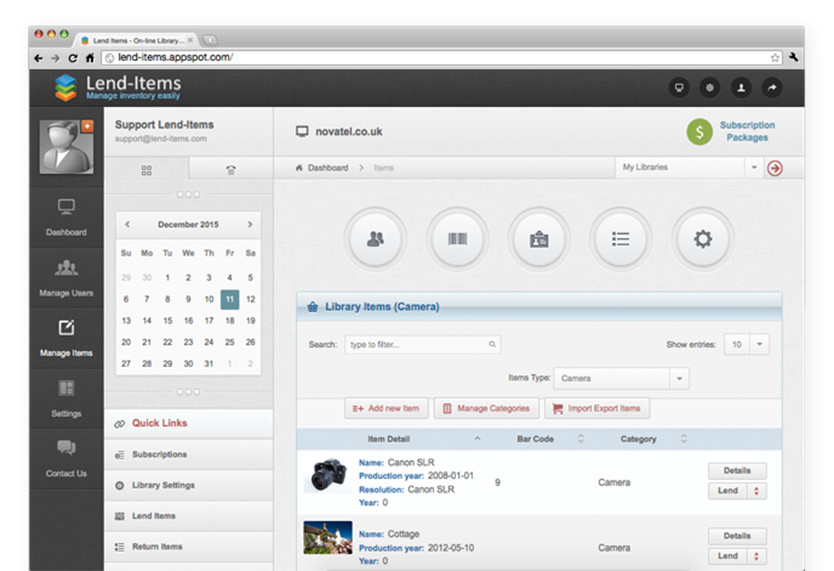
\includegraphics[width=0.7\textwidth]{figura1.jpg}
	\source[\citeonline{DepEngEle}.]
	\label{fig:label_da_figura}
\end{figure}


\begin{figure}[!h]
	\centering
	\caption{Pode-se verificar quais são as pessoas que utilizam a plataforma.}
	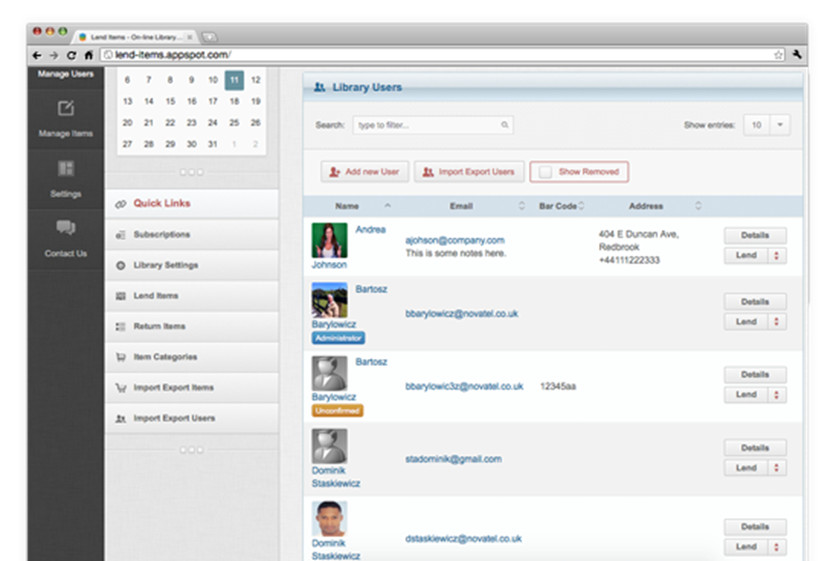
\includegraphics[width=0.7\textwidth]{figura2.jpg}
	\source[\citeonline{DepEngEle}.]
	\label{fig:label_da_figura}
\end{figure}

Outras plataformas que podemos ter como base são Vaivem, apresentando a seguinte interface:

\begin{figure}[!h]
	\centering
	\caption{Interface de Vaivem.}
	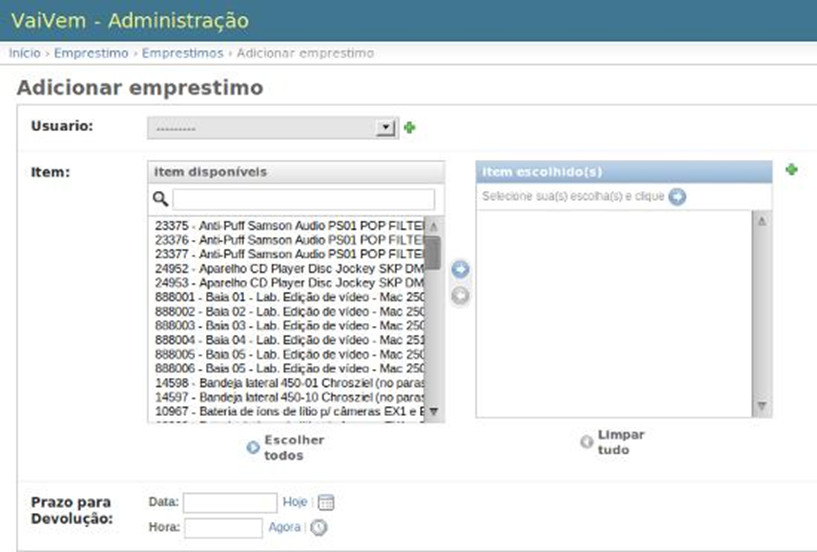
\includegraphics[width=0.7\textwidth]{figura3.jpg}
	\source[\citeonline{DepEngEle}.]
	\label{fig:label_da_figura}
\end{figure}


Há outros softwares também como Software de Controle de UPJ e TotalLoc.
Também estamos utilizando o seguinte modelo de banco de dados para nosso projeto :
\begin{figure}[!h]
	\centering
	\caption{Configuração do Banco de Dados.}
	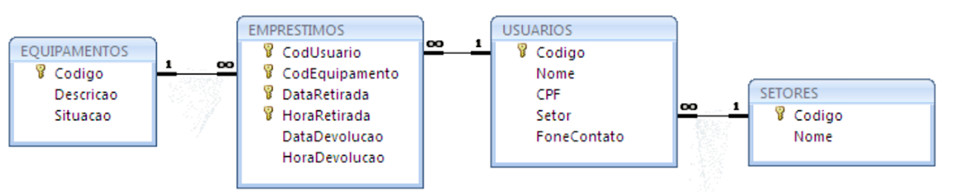
\includegraphics[width=0.7\textwidth]{figura4.jpg}
	\source[\citeonline{DepEngEle}.]
	\label{fig:label_da_figura}
\end{figure}


Também podemos ver quando o banco é acessado pelo seguintes esquemático:

\begin{figure}[!h]
	\centering
	\caption{Acesso do Banco de Dados.}
	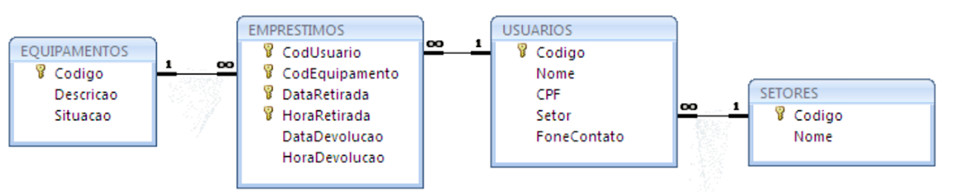
\includegraphics[width=0.7\textwidth]{figura4.jpg}
	\source[\citeonline{DepEngEle}.]
	\label{fig:label_da_figura}
\end{figure}


\chapter[Cronograma de execução]{Cronograma de execução}
% Ajustar esse \vspace de acordo com o necessário
\vspace{-42pt}
Teste de citação: \cite{DepEngEle}


\chapter[Alocação de recursos
]{Alocação de recursos}
% Ajustar esse \vspace de acordo com o necessário
\vspace{-42pt}
Teste de citação: \cite{DepEngEle}


% --------------------------------------------------- %
%				Elementos Pós-Textuais				  %
% --------------------------------------------------- %

\postextual

% --------------------------------------------------- %
%				Referências Bibliográficas		      %
% --------------------------------------------------- %

\bibliographystyle{abntex2-alf} % Autor-Data
\renewcommand{\bibname}{Referências Bibliográficas}
\bibliography{bibliografia}

% --------------------------------------------------- %
%						Apêndices				  	  %
% --------------------------------------------------- %

\begin{apendicesenv}
% Imprime uma página indicando o início dos apêndices
\partapendices

% Insira os apêndices aqui em forma de capítulos

\end{apendicesenv}

% --------------------------------------------------- %
%						Anexos						  %
% --------------------------------------------------- %

\begin{anexosenv}
%
%% Imprime uma página indicando o início dos anexos
\partanexos

\end{anexosenv}

% --------------------------------------------------- %
%					Índice Remissivo				  %
% --------------------------------------------------- %
\phantompart
\printindex

\end{document}
